% Pipeline: TikZ swimlanes, no icons. Counts from paper/result.md (R1, R3-R5).
% Shared setup for the diagrams (teaser, pipeline, worked). Built with XeLaTeX so that all text is Arial, in black.
% Sizes match the paper's acmart sigconf sizes (\footnotesize 7 pt); the smallest text is 6 pt.
\documentclass[border=0.5pt]{standalone}
\usepackage{fontspec}
\setmainfont{Arial}\setsansfont{Arial}\setmonofont{Menlo}[Scale=MatchLowercase]
\usepackage{unicode-math}\setmathfont{FiraMath-Regular.otf}
\usepackage{booktabs}
\usepackage{tikz}
\usetikzlibrary{arrows.meta,calc,positioning,fit,backgrounds,shapes.geometric}
\renewcommand\large{\fontsize{10}{12}\selectfont}
\renewcommand\small{\fontsize{8}{10}\selectfont}
\renewcommand\footnotesize{\fontsize{7}{8.4}\selectfont}
\renewcommand\scriptsize{\fontsize{6.5}{7.6}\selectfont}
\renewcommand\tiny{\fontsize{6}{7}\selectfont}
\newcommand{\nohyph}{\hyphenpenalty=10000\exhyphenpenalty=10000\relax}
\newcommand{\sql}[1]{\texttt{#1}}
% the edited SQL clause, highlighted as in AMBROSIA and the test-suite paper; plain check and cross marks
\newcommand{\hl}[2]{{\setlength{\fboxsep}{0.7pt}\colorbox{#1f}{\vphantom{Ay}\texttt{#2}}}}
\newfontfamily\markfont{Arial Unicode MS}\newcommand{\yes}{{\markfont ✓}}\newcommand{\no}{{\markfont ✗}}
% math letters in Arial italic; the open-request circle is drawn; only the arrow comes from Fira Math
\newcommand{\vq}[1]{\textit{q}\textsubscript{#1}}\newcommand{\vp}[1]{\textit{p}\textsubscript{#1}}\newcommand{\vo}{\mbox{\textit{q}\hspace{0.3pt}\raisebox{-0.25ex}{\tikz[baseline=0pt]\draw[line width=0.45pt] (0,1.1pt) circle (1.1pt);}}}
% box lines: A (blue) and B (orange) as in the data figures; neutral lines grey. Text is always black.
% colors as in AMBROSIA's and AmbiQT's diagrams (draw.io palette): interpretation A blue, interpretation B orange, code blocks light gray
\definecolor{sbA}{HTML}{6C8EBF}\definecolor{sbB}{HTML}{D79B00}\definecolor{sbAf}{HTML}{DAE8FC}\definecolor{sbBf}{HTML}{FFE6CC}\definecolor{sbline}{HTML}{4D4D4D}
\definecolor{sbfill}{HTML}{F5F5F5}

\begin{document}
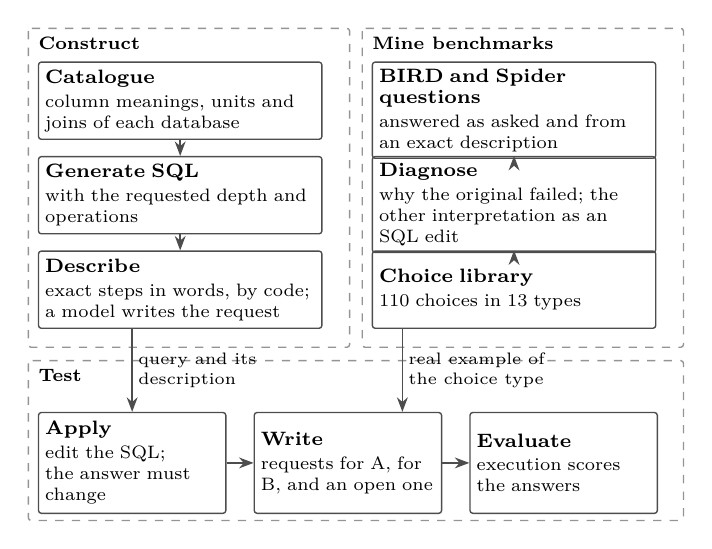
\begin{tikzpicture}[x=1cm, y=1cm, font=\scriptsize, >=Stealth, line width=0.5pt,
  lane/.style={draw=sbline!60, dashed, rounded corners=1pt},
  lt/.style={font=\scriptsize\bfseries, text=black, anchor=north west, inner sep=0pt},
  st/.style={execute at begin node=\nohyph, draw=sbline, rounded corners=1pt, inner sep=2.4pt, align=left, text width=3.43cm, minimum height=0.98cm, anchor=north west},
  bt/.style={execute at begin node=\nohyph, draw=sbline, rounded corners=1pt, inner sep=2.4pt, align=left, text width=2.21cm, minimum height=1.28cm, anchor=north west},
  arr/.style={->, draw=sbline}]
\newcommand{\hd}[1]{\textbf{\footnotesize #1}\\[1pt]}
% ---- lanes
\draw[lane] (0,0) rectangle (4.08,-4.05);   \node[lt] at (0.12,-0.1) {Construct};
\draw[lane] (4.24,0) rectangle (8.32,-4.05); \node[lt] at (4.36,-0.1) {Mine benchmarks};
\draw[lane] (0,-4.22) rectangle (8.32,-6.25); \node[lt] at (0.12,-4.32) {Test};
% ---- construct
\node[st] (c1) at (0.12,-0.42) {\hd{Catalogue}column meanings, units and joins of each database};
\node[st] (c2) at (0.12,-1.62) {\hd{Generate SQL}with the requested depth and operations};
\node[st] (c3) at (0.12,-2.82) {\hd{Describe}exact steps in words, by code; a model writes the request};
% ---- mine
\node[st] (m1) at (4.36,-0.42) {\hd{BIRD and Spider questions}answered as asked and from an exact description};
\node[st] (m2) at (4.36,-1.62) {\hd{Diagnose}why the original failed; the other interpretation as an SQL edit};
\node[st] (m3) at (4.36,-2.82) {\hd{Choice library}110 choices in 13 types};
\foreach \a/\b in {c1/c2, c2/c3, m1/m2, m2/m3} \draw[arr] (\a.south) -- (\b.north);
% ---- test
\node[bt] (t1) at (0.12,-4.87) {\hd{Apply}edit the SQL; the answer must change};
\node[bt] (t2) at (2.86,-4.87) {\hd{Write}requests for A, for B, and an open one};
\node[bt] (t3) at (5.6,-4.87) {\hd{Evaluate}execution scores the answers};
\draw[arr] (t1.east) -- (t2.west); \draw[arr] (t2.east) -- (t3.west);
\draw[arr] (c3.south -| t1.north) -- node[right, font=\tiny, inner sep=2pt, align=left] {query and its\\description} (t1.north);
\draw[arr] (4.75,0 |- m3.south) -- node[right, font=\tiny, inner sep=2pt, align=left] {real example of\\the choice type} (4.75,0 |- t2.north);
\end{tikzpicture}
\end{document}
